% Archivo: examples.tex


\section{Primera parte con `\texttt{tcolorbox}'}

\lipsum[2]

% Default tcolorbox
\begin{tcolorbox}[colback=main!5!white, colframe=main!75!black, title=\textbf{Definición con código}, toptitle=1.5mm, bottomtitle=1.5mm, breakable]
    \lipsum[2] \begin{align*}
        y_t = \beta_0 + \beta_1 x_t + \beta_2 x_{t-1} + \beta_3 x_{t-2} + \beta_4 x_{t-3} + \varepsilon_t
    \end{align*}
    Esto luce de la siguiente manera en R:
    \begin{lstlisting}[style=R]
# Código en R
y <- c(1, 2, 3, 4, 5)
x <- c(1, 2, 3, 4, 5)
lm(y ~ x)
    \end{lstlisting}
    
\end{tcolorbox}

% Secondary tcolorbox
\begin{tcolorbox}[colback=secondary!5!white, colframe=secondary!75!black, title=\textbf{Nota con código}, toptitle=1.5mm, bottomtitle=1.5mm, breakable]
    \lipsum[3] \begin{align*}
        y_t = \beta_0 + \beta_1 x_t + \beta_2 x_{t-1} + \beta_3 x_{t-2} + \beta_4 x_{t-3} + \varepsilon_t
    \end{align*}
    Esto luce de la siguiente manera en R:
    \begin{lstlisting}[style=R]
# Código en R
y <- c(1, 2, 3, 4, 5)
x <- c(1, 2, 3, 4, 5)
lm(y ~ x)
    \end{lstlisting}

    \tcbsubtitle{Subtítulo de la caja}
    \lipsum[4]

    \tcblower
    \lipsum[5]

\end{tcolorbox}

% Example tcolorbox
\begin{tcolorbox}[colback=tertiary!5!white, colframe=tertiary!75!black, title=\textbf{Ejemplo con Código}, toptitle=1.5mm, bottomtitle=1.5mm, breakable]
    \lipsum[6] \begin{align*}
        y_t = \beta_0 + \beta_1 x_t + \beta_2 x_{t-1} + \beta_3 x_{t-2} + \beta_4 x_{t-3} + \varepsilon_t
    \end{align*}
    \lipsum[7]
\end{tcolorbox}

\section{Gráficas}

\begin{multicols}{2}
        
    \begin{figure}[H]
        % If you want to resize to textwidth use \textwidth:
        \centering
        \resizebox{6cm}{!}{
        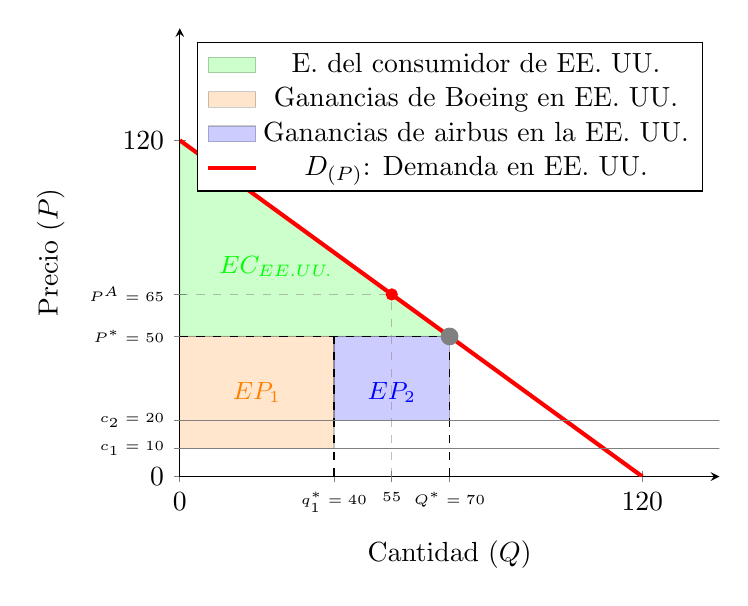
\begin{tikzpicture}
            \begin{axis}[
                axis lines = left,
                xlabel = Cantidad ($Q$),
                ylabel = Precio ($P$),
                % Mostrar valores cada 120:
                xtick distance = 120,
                ytick distance = 120,
                xmin = 0, xmax = 140,
                ymin = 0, ymax = 160,
                legend pos = north east,
                extra y ticks={10, 20, 50, 65},
                extra y tick labels={\tiny{$c_1 = 10$}, \tiny{$c_2 = 20$}, \tiny{$P^*=50$}, \tiny{$P^A=65$}},
                extra x ticks={40, 55, 70},
                extra x tick labels={\tiny{$q_1^*=40$}, \tiny{$55$}, \tiny{$Q^*=70$}},
            ]

            % Excedente del consumidor
            \draw [fill=green, opacity=0.2] (0, 50) -- (0, 120) -- (70, 50) -- cycle;
            \addlegendimage{area legend, opacity=0.2, fill=green} \addlegendentry{E. del consumidor de EE. UU.}
            \node[color=green] at (axis cs: 25, 75) {\small{$EC_{\text{EE. UU.}}$}};

            % % Excedente del productor (Boeing)
            \draw [fill=orange, opacity=0.2] (0, 10) -- (0, 50) -- (40, 50) -- (40, 10) -- cycle;
            \addlegendimage{area legend, opacity=0.2, fill=orange} \addlegendentry{Ganancias de Boeing en EE. UU.}
            \node[color=orange] at (axis cs: 20, 30) {\small{$EP_1$}};

            % Excedente del productor (Airbus)
            \draw [fill=blue, opacity=0.2] (40, 20) -- (40, 50) -- (70, 50) -- (70, 20) -- cycle;
            \addlegendimage{area legend, opacity=0.2, fill=blue} \addlegendentry{Ganancias de airbus en la EE. UU.}
            \node[color=blue] at (axis cs: 55, 30) {\small{$EP_2$}};

            % Curva de demanda
            \addplot [
                domain=0:120, 
                samples=200, 
                color=red,
                line width=1.5pt,
            ]
            {120 - x};
            \addlegendentry{$D_{(P)}$: Demanda en EE. UU.}

            % Marcas
            \addplot [forget plot,only marks, mark = *, mark size = 3pt, color = gray] coordinates {(70, 50)};
            % Vertical 1
            \addplot [
                forget plot,
                color=black,
                line width=0.5pt,
                dashed
            ] coordinates {(40, 0) (40, 50)};
            % Vertical 2
            \addplot [
                forget plot,
                color=black,
                line width=0.5pt,
                dashed
            ] coordinates {(70, 0) (70, 50)};
            % Horizontal 1
            \addplot [
                forget plot,
                color=black,
                line width=0.5pt,
                dashed
                ] coordinates {(0, 50) (70, 50)};

            % Vertical autarquía
            \addplot [
                forget plot,
                color=gray,
                opacity=0.5,
                line width=0.5pt,
                dashed
            ] coordinates {(55, 0) (55, 65)};
            % Horizontal autarquía
            \addplot [
                forget plot,
                color=gray,
                opacity=0.5,
                line width=0.5pt,
                dashed
            ] coordinates {(0, 65) (55, 65)};
            % Equilibrio autarquía
            \addplot [forget plot,only marks, mark = *, mark size = 2pt, color = red,] coordinates {(55, 65)};

            % Coste marginal
            % Boeing
            \addplot [
                forget plot,
                domain=0:200, 
                samples=200, 
                color=gray,
                line width=0.5pt,
            ]
            {10};
            % Airbus
            \addplot [
                forget plot,
                domain=0:200, 
                samples=200, 
                color=gray,
                line width=0.5pt,
            ]
            {20};

            % % Ingreso marginal
            % \addplot [
            %     forget plot,
            %     domain=0:120, 
            %     samples=200, 
            %     color=gray,
            %     line width=0.5pt,
            %     dashed,
            %     opacity=0.5,
            % ]
            % {120 - 2*x};
            \end{axis}
        \end{tikzpicture}
        }
        \caption{Equilibrio en condiciones de libre comercio en EE. UU.}
    \end{figure}

    \begin{figure}[H]
        % If you want to resize to textwidth use \textwidth:
        \centering
        \resizebox{7cm}{!}{
        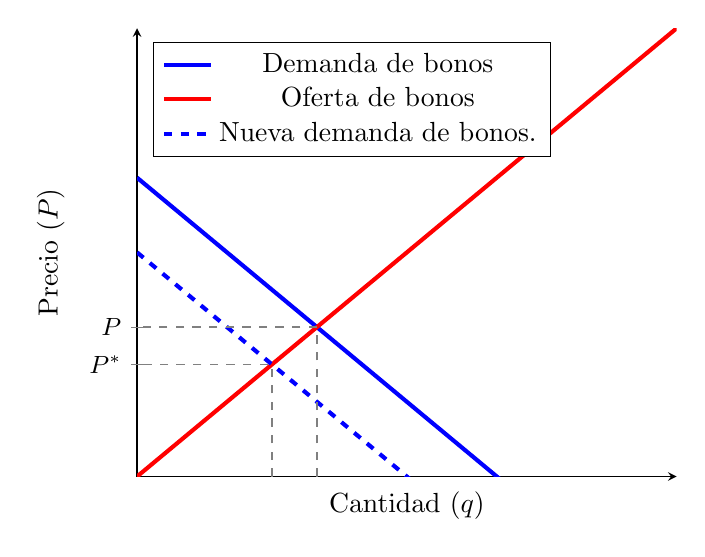
\begin{tikzpicture}
            \begin{axis}[
                axis lines = left,
                xlabel = Cantidad ($q$),
                ylabel = Precio ($P$),
                xmin = 0, xmax = 6,
                ymin = 0, ymax = 6,
                legend pos = north west,
                % Ocultar ticks:
                xtick=\empty,
                ytick=\empty,
                % more labels in y axis:
                extra y ticks={2, 1.5},
                extra y tick labels={\small{$P$}, \small{$P^*$}},
            ]
            \addplot [
                domain=0:10, 
                samples=100, 
                color=blue,
                line width=1.5pt,
            ]
            {4 - x};
            \addlegendentry{Demanda de bonos};
            \addplot [
                domain=0:10, 
                samples=100, 
                color=red,
                line width=1.5pt,
            ]
            {x};
            \addlegendentry{Oferta de bonos};
            % Desplazamiento de la demanda:
            \addplot [
                domain=0:10, 
                samples=100, 
                color=blue,
                line width=1.5pt,
                dashed,
            ]
            {3 - x};
            \addlegendentry{Nueva demanda de bonos.};
            % Líneas punteadas:
            \draw[dashed, color=gray, line width=0.5pt] (2,0) -- (2,2) -- (0,2); % Original
            \draw[dashed, color=gray, line width=0.5pt] (1.5,0) -- (1.5,1.5) -- (0,1.5); % Nuevo
            \end{axis}
        \end{tikzpicture}
        }
        \caption{\textit{Equilibrio de mercado}. La demanda baja, lo que hace bajar los precios.}
    \end{figure}

    \columnbreak

    \begin{figure}[H]
        % If you want to resize to textwidth use \textwidth:
        \centering
        \resizebox{6cm}{!}{
        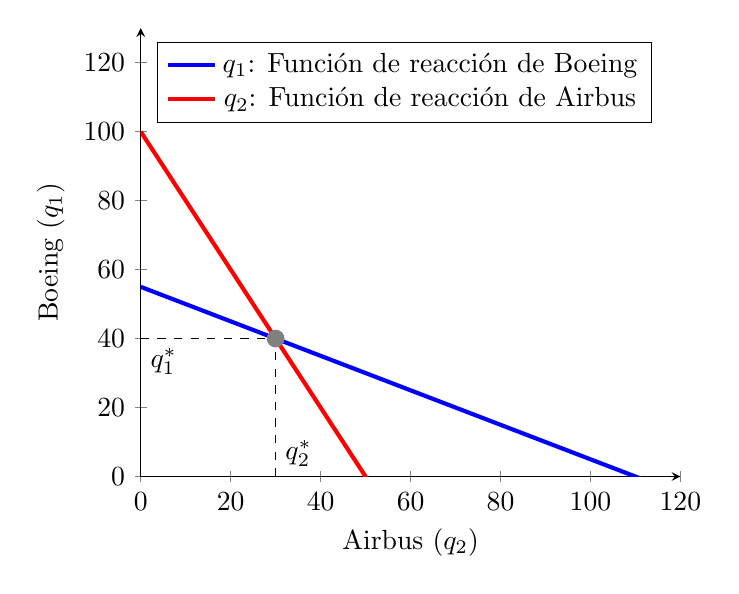
\begin{tikzpicture}
            \begin{axis}[
                axis lines = left,
                xlabel = Airbus ($q_2$),
                ylabel = Boeing ($q_1$),
                xmin = 0, xmax = 120,
                ymin = 0, ymax = 130,
                legend pos = north west,
            ]
            \addplot [
                domain=0:120, 
                samples=200, 
                color=blue,
                line width=1.5pt,
            ]
            {55 - x/2};
            \addlegendentry{$q_1$: Función de reacción de Boeing}
            \addplot [
                domain=0:120, 
                samples=200, 
                color=red,
                line width=1.5pt,
            ]
            {100 - 2*x};
            \addlegendentry{$q_2$: Función de reacción de Airbus}
            \addplot [forget plot,only marks, mark = *, mark size = 3pt, color = gray] coordinates {(30, 40)};
            \addplot [
                forget plot,
                color=black,
                line width=0.5pt,
                dashed
            ] coordinates {(30, 0) (30, 40)};
            \node[above right] at (axis cs: 30, 0) {$q_2^*$};
            \addplot [
                forget plot,
                color=black,
                line width=0.5pt,
                dashed
            ] coordinates {(0, 40) (30, 40)};
            \node[below right] at (axis cs: 0, 40) {$q_1^*$};
            \end{axis}
        \end{tikzpicture}
        }
        \caption{Funciones de reacción de Boeing y Airbus en EE. UU.}
    \end{figure}

    \begin{figure}[H]
        % If you want to resize to textwidth use \textwidth:
        \centering
        \resizebox{6cm}{!}{
        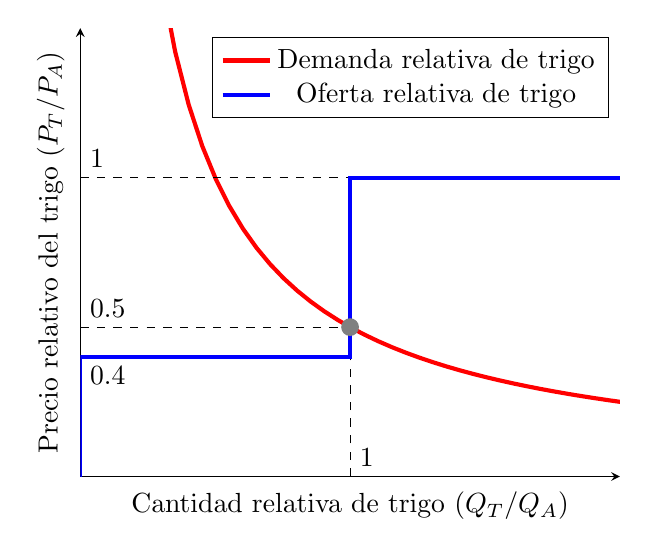
\begin{tikzpicture}
            \begin{axis}[
                axis lines = left,
                xlabel = Cantidad relativa de trigo ($Q_T/Q_A$),
                ylabel = Precio relativo del trigo ($P_T/P_A$),
                xmin = 0, xmax = 2,
                ymin = 0, ymax = 1.5,
                % legend pos = north west,
                xtick = \empty,
                ytick = \empty,
            ]
            \addplot [
                domain=0:10, 
                samples=200, 
                color=red,
                line width=1.5pt,
            ]
            {1/(2*x)};
            \addlegendentry{Demanda relativa de trigo}
            % To add a equilibrium in (0.4, 1.25):
            \addplot [forget plot,only marks, mark = *, mark size = 3pt, color = gray] coordinates {(1, 0.5)};
            % To add a line from axis to equilibrium:
            \addplot [forget plot,dashed, color = black] coordinates {(1, 0) (1, 0.4)};
            \addplot [forget plot,dashed, color = black] coordinates {(0, 0.5) (1, 0.5)};
            \addplot [forget plot,dashed, color = black] coordinates {(0, 1) (1, 1)};
            % To add value to the axis:
            \node[above right] at (axis cs: 1, 0) {1};
            \node[above right] at (axis cs: 0, 1) {1};
            \node[below right] at (axis cs: 0, 0.4) {0.4};
            \node[above right] at (axis cs: 0, 0.5) {0.5};
            % Relative offer:
            % \addplot [
            %     forget plot,
            %     color=blue,
            %     line width=3pt,
            % ] coordinates {(0, 0) (0, 0.4)};
            % \addplot [
            %     color=blue,
            %     line width=1.5pt,
            % ] coordinates {(0, 0.4) (0.9, 0.4)};
            % \addplot [
            %     forget plot,
            %     color=blue,
            %     line width=1.5pt,
            % ] coordinates {(0.9, 0.4) (0.9, 1)};
            % \addplot [
            %     color=blue,
            %     line width=1.5pt,
            % ] coordinates {(0.9, 1) (2, 1)};
            % En una sola línea:
            \addplot [
                color=blue,
                line width=1.5pt,
            ] coordinates {(0, 0) (0, 0.4) (1, 0.4) (1, 1) (2, 1)};
            \addlegendentry{Oferta relativa de trigo}
            \end{axis}
        \end{tikzpicture}
        }
        \caption{Equilibrio mundial en condiciones de libre comercio}
    \end{figure}

\end{multicols}

\section{Experimentales}
% \addcontentsline{toc}{subsection}{Ejemplo de \box}

\begin{tcolorbox}[colback=main!5!white, colframe=main!75!black, title=\textbf{Ejemplo de Código}, toptitle=1.5mm, bottomtitle=1.5mm, breakable]

    \lipsum[10] \begin{align*}
        y_t = \beta_0 + \beta_1 x_t + \beta_2 x_{t-1} + \beta_3 x_{t-2} + \beta_4 x_{t-3} + \varepsilon_t
    \end{align*}
    \lipsum[11]

\end{tcolorbox}

\HRuleGray

\lipsum[12]